% 2013 年春季上海卷第 9 题：正方体 ABCD-A1B1C1D1
% 突出异面直线 A1B 与 B1C；图中透视比例不代表题设尺寸。
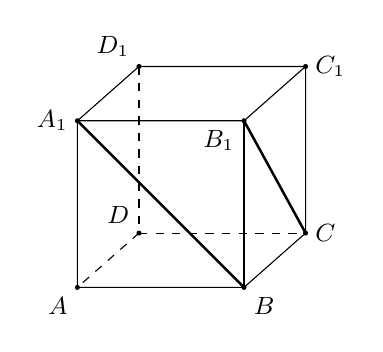
\begin{tikzpicture}[>=stealth, scale=0.92, font=\small]
  \coordinate (A)  at (0,0);
  \coordinate (B)  at (2.30,0);
  \coordinate (C)  at (3.15,0.75);
  \coordinate (D)  at (0.85,0.75);
  \coordinate (A1) at (0,2.30);
  \coordinate (B1) at (2.30,2.30);
  \coordinate (C1) at (3.15,3.05);
  \coordinate (D1) at (0.85,3.05);
  % 可见棱
  \draw (A) -- (B) -- (C) -- (C1) -- (B1) -- (A1) -- cycle;
  \draw (A1) -- (D1) -- (C1);
  \draw (B) -- (B1);
  % 不可见棱
  \draw[dashed] (D1) -- (D);
  \draw[dashed] (D) -- (C);
  \draw[dashed] (D) -- (A);
  % 异面直线 A1B 与 B1C
  \draw[line width=0.9pt] (A1) -- (B);
  \draw[line width=0.9pt] (B1) -- (C);
  % 顶点
  \fill (A) circle (1pt) node[below left] {$A$};
  \fill (B) circle (1pt) node[below right] {$B$};
  \fill (C) circle (1pt) node[right] {$C$};
  \fill (D) circle (1pt) node[above left] {$D$};
  \fill (A1) circle (1pt) node[left] {$A_1$};
  \fill (B1) circle (1pt) node[below left] {$B_1$};
  \fill (C1) circle (1pt) node[right] {$C_1$};
  \fill (D1) circle (1pt) node[above left] {$D_1$};
\end{tikzpicture}
